\subsection{Launcher}

    \vspace{0.5cm}
    \subsubsection{Première soutenance}
    \vspace{0.5cm}

        Une première version du lanceur a été créée avec le Framework Avalonia, qui permet de développer 
        en C\#, mais utilise beaucoup de librairies externes sous forme de fichiers dll qui alourdissent 
        énormément le fichier d'installation (plus de 300 Mo). Pour créer l'installer du launcher, nous 
        avons utilisé le classique Inno Setup, qui est un logiciel permettant de packer un exécutable et 
        toutes ses dépendances dans un fichier d'installation. 

        \begin{figure}[hbt!]
            \centering
            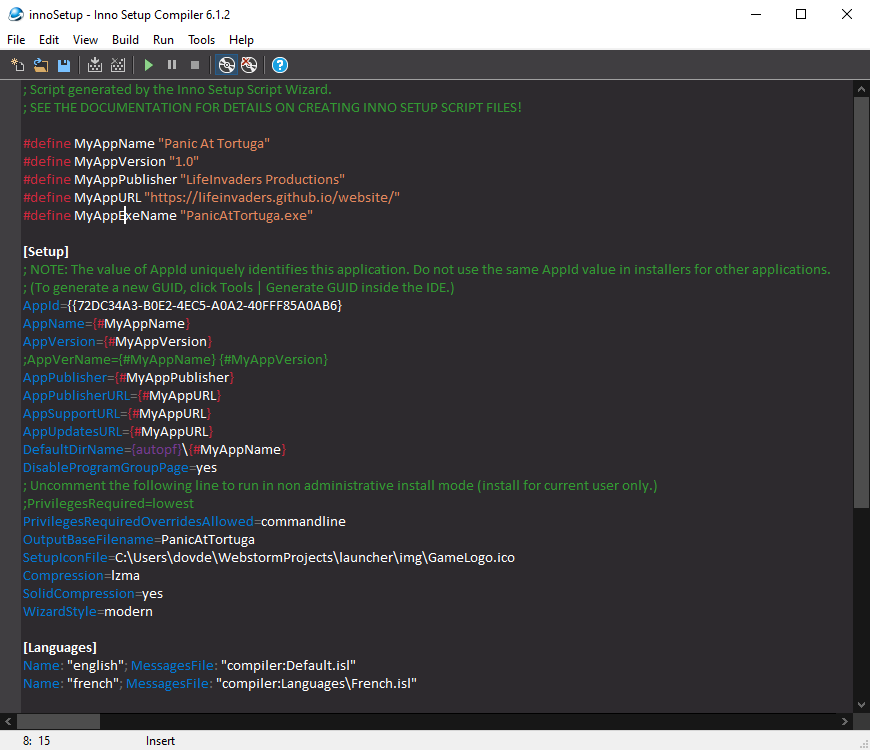
\includegraphics[scale=0.48]{innosetup.png}
            \caption{Fichier de configuration de Inno Setup}
        \end{figure}

        Le fichier de configuration permet d'indiquer la source (dossier contenant le launcher Avalonia), la destination, 
        l'icône de l'installer, et éventuellement des informations pour l'uninstaller.

    \vspace{0.5cm}
    \subsubsection{Deuxième soutenance}
    \vspace{0.5cm}

        Le lanceur du jeu est un élément crucial, car il permet d'installer 
        le jeu et de le maintenir à jour. Une première version du launcher avait 
        été créée avec Avalonia, un Framework C\#. Cependant, il faisait appel à des 
        librairies externes, ce qui l'alourdissait et rendait son fonctionnement instable. 
        C'est pour cette raison que nous avons décidé, pour la deuxième soutenance, de nous 
        tourner vers le Framework Electron, qui est parfaitement compatible avec toutes les 
        plateformes car il repose sur du HTML.

        \begin{figure}[hbt!]
            \centering
            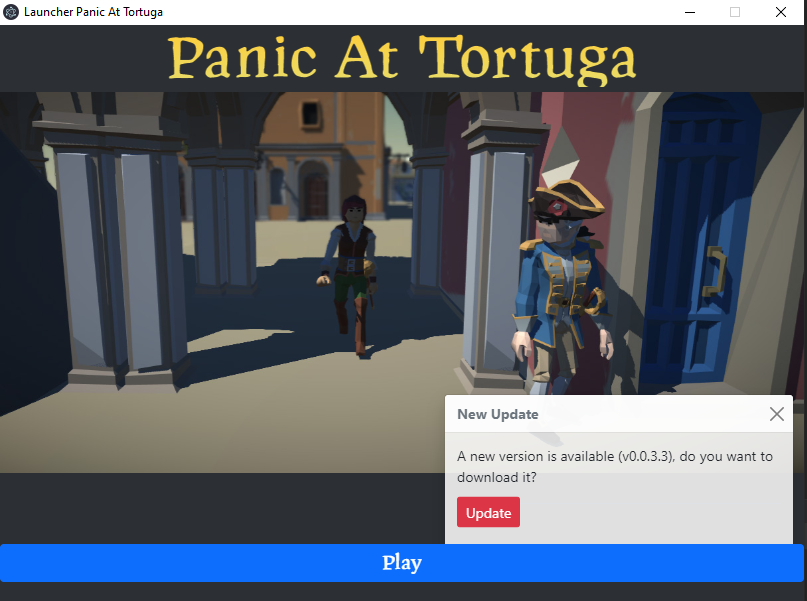
\includegraphics[scale=0.52]{launcher.png}
            \caption{Aperçu du Launcher}
        \end{figure}
        \FloatBarrier

        Le lanceur du jeu sous Electron est capable de se connecter au repo Github et de récupérer la 
        dernière version du jeu afin de la comparer à la version actuelle pour proposer de télécharger les nouveautés. 
        Cela permet de constamment maintenir le jeu à jour, pour éviter des conflits de versions 
        ou toutes autres erreurs. Le html utilisé permet aussi de s'adapter parfaitement à toutes les formes de 
        fenêtres sans problèmes d'échelles ou d'overlay.

    \vspace{0.5cm}
    \subsubsection{Dernière soutenance}
    \vspace{0.5cm}

        Du côté d'\textit{Inno Setup}, nous avons dû faire quelques ajustements pour que l'uninstaller supprime le dossier 
        contenant le jeu (en plus de celui du lanceur), et nous avons utilisé Resource Hacker (ResHack) pour modifier l'icône 
        du launcher, afin qu'elle apparaisse après installation au lieu de l'icone Electron.

        Des bugs au lancement avaient également lieu, notamment concernant le fichier version.json qui enregistre la version actuelle du jeu, 
        et au niveau du chemin de l'exécutable, que nous avons dû modifier.
    

